\section{Plasticity}
\label{sec:plasticity}

Plasticity or more specific \emph{neuroplasticity}, when it comes to brains, is the ability of the brain to change its neuronal structure depending on experience. It can be separated in \emph{functional plasticity} and \emph{structural plasticity}.

\begin{itemize}
\item Functional plasticity: Changes in synaptic transmission characteristics due to changes in amount of neurotransmitter or receptors
\item Structural plasticity: Changes in structure of the neuron, like growing or shrinking of axons, dendrites, synapses or even whole neurons
\end{itemize}

Furthermore, \emph{synaptic plasticity} describes all processes related to synapses, like changes in transmission characteristics and growing or shrinking of synapses. Regarding synaptic plasticity one can distinguish between \emph{pre-synaptic plasticity} and \emph{post-synaptic plasticity}. Pre-synaptic plasticity means, that the amount of released neurotransmitters or the time for readmission of neurotransmitters changes. Post-synaptic plasticity changes the sensibility for a given amount of neurotransmitters. For example the amount of receptors (ion channels) can be adapted. Furthermore, plasticity can vary in duration. \emph{Short-term plasticity} changes the transmission characteristic of the synapses in a scale of milliseconds to minutes, while \emph{long-term plasticity} has an effect for hours, or even years. Both can be separated in so called depression --- \acf{std} and \acf{ltd} --- which means a decrease in connectivity, and potentiation --- \acf{stp} and \acf{ltp} --- which means an increase in connectivity between the synapses.

Second messengers (see above in section \ref{sec:synapse}) play an important role in synaptic plasticity \parencite{skrebitskiui1999synaptic}. Metabotropic receptors can not only start mechanisms to open ion channels, they can also start processes to change the behavior of receptors, channels or neurotransmitters.

In artificial neural networks the synaptic transmission characteristic can be modeled as a weight $w_{ij}$ between neuron $i$ and neuron $j$, as already used in equation \eqref{eq:activation}. If there is no connection between two neurons, it holds that $w_{ij} = 0$. Functional plasticity corresponds to a change in $w_{ij} \in (0,1]$, indicated as $\Delta w_{ij}$, whereby structural plasticity sets the weight to zero or non-zero.

\subsection{Hebb's rule}

A rule that simplifies a functional plasticity mechanism is the \emph{Hebb rule}. Biologically, synapses strengthen their connection if the firing of neuron $j$ and the firing of neuron $i$ is close together. In that case the weight $w_{ij}$ will increase.

\begin{figure}[!b]
	\centering
	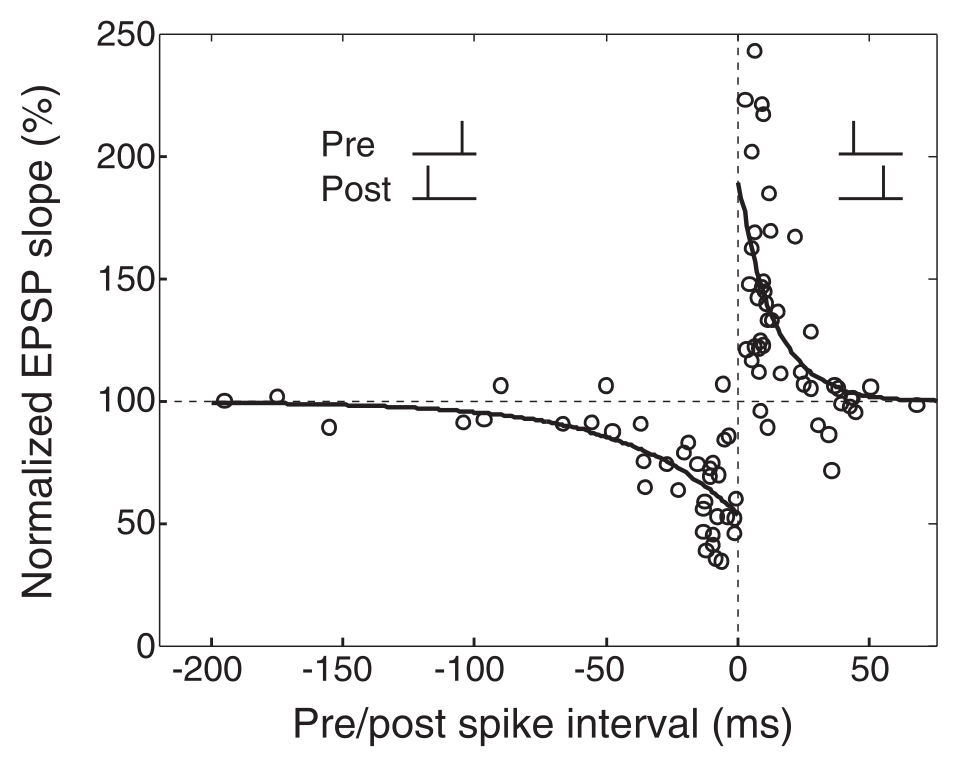
\includegraphics[width=0.6\textwidth]{neurons_plasticity/stdp.png}
	\caption[Spike-timing-dependent plasticity]{Spike-timing-dependent plasticity \parencite[figure 1]{dan2006spike}. The closer the post-synaptic neuron spikes before the pre-synaptic neuron spikes, the higher will be the \emph{decrease} in weight and vice versa.}
	\label{fig:stdp}
\end{figure}

For artificial neural networks holds therefore

\begin{equation}
\Delta w_{ij} = \eta \cdot z_j \cdot a_i,
\end{equation}

where $\eta$ is a learning rate. A high learning rate results in fast but inaccurate convergence, while a low learning rate results in slow but accurate convergence.

\subsection{Spike-timing-dependent plasticity}

The \acfi{stdp} is a causal type of Hebb's rule, depending on temporal correlations between the spikes of pre-synaptic and post-synaptic neurons \parencite{sjostrom2010spike}. Spikes arriving repeatedly at the pre-synapses, some time before or after an action potential at the post-synaptic neuron, lead to long-term plasticity. In case that spikes arrive shortly before an action potential of the post-synaptic neuron, it leads to \acl{ltp}. In case that spikes arrive shortly after an action potential of the post-synaptic neuron, it leads to \acl{ltd}. The time scale where plasticity occurs, varies between different types of synapses. In most cases it is of the order of milliseconds \parencite{dan2006spike}. An illustration of the \acs{stdp} is shown in figure \ref{fig:stdp}.

\begin{wrapfigure}{R}{0.45\textwidth}
	\centering
	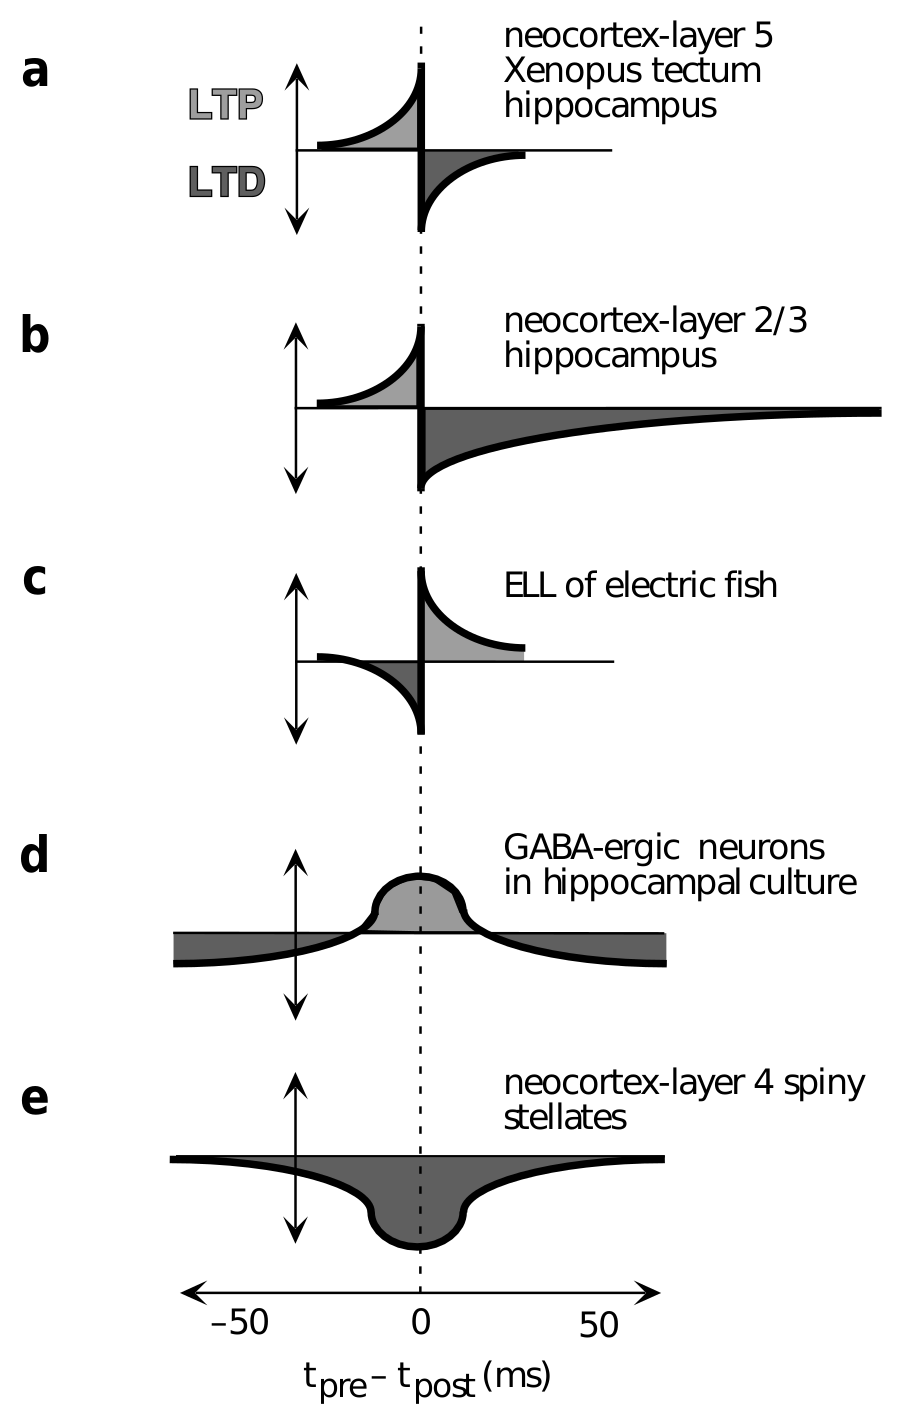
\includegraphics[width=0.45\textwidth]{neurons_plasticity/learning-window.png}
	\caption[Learning windows]{\ac{stdp} learning windows \parencite[figure 2]{abbott2000synaptic}.}
    \label{fig:learning-windows}
    \vspace{-10pt}
\end{wrapfigure}

A mathematically formulation of the \ac{stdp} was done by \textcite{sjostrom2010spike} and more specific by \textcite{kempter1999hebbian}. Consider a post-synaptic neuron with activity $x_i(t)$ and a pre-synaptic neuron with activity $x_j(t)$. Assume many spikes at the post-synaptic neuron, counted by $l \in \{ 1,...,n_l \}$, where $n_l$ is the total number of spikes. $t_i^l$ indicates the time for every spike at neuron $i$ with $x_i(t_i^l) = 1$. Furthermore, the number of spikes of the pre-synaptic neurons is counted by $k \in \{ 1,...,n_k \}$, where $n_k$ is the total number of spikes. $t_j^k$ indicates the points in time at which the pre-synaptic neuron is firing with $x_j(t_j^k) = 1$.

The \emph{learning window} is a function $f(\Delta t)$, where $\Delta t = t_j^k - t_i^l$. It can be defined in various ways, some are shown in figure \ref{fig:learning-windows}. Using the learning window, the change of the weight can be defined as

\begin{equation}
\label{eq:stdp-orig}
\Delta w_{ij} = \sum_{k=1}^{n_k} \sum_{l=1}^{n_l} f(\Delta t) = \sum_{k=1}^{n_k} \sum_{l=1}^{n_l} f(t_j^k - t_i^l).
\end{equation}

$f(\Delta t)$ is often chosen as an exponential function \parencite{sjostrom2010spike}. It could be shown, that an exponential learning window is able to model experimental findings \parencite{zhang1998critical}. It can be defined as

\begin{equation}
f(\Delta t) = \begin{cases}
\;A_+ \exp(-\Delta t / \tau_+), & x > 0\\
\;-A_- \exp(\Delta t / \tau_-), & x < 0
\end{cases},
\end{equation}

where $A_+$ and $A_-$ are parameters to choose. $\tau_+$ and $\tau_-$ are time constants and often chosen as $\tau_+ = \tau_- = 10\,ms$.

If, for the exponential learning window, $t_j^k$ and $t_i^l$ are close to each other most of the time, which means that pre- and post-synaptic neurons spiking in succession, there will be a change in the weight between those neurons, depending on the sign. The more often those neurons fire close to each other, the higher will be the sum and the change of the weight. The principle of the exponential learning window is shown in figure \ref{fig:learning-windows}a.

For simulations of neural networks which are focused on more high level network based research, \ac{stdp} is often modeled more simple. One simplified version, where the weight only depends on the spiking between two discrete time steps, will be introduced in section \ref{sec:sorn}.

\subsection{Homeostatic plasticity}

A network just processing Hebb's rule would soon end in a destabilized state. If \acs{ltp} becomes dominant, the synapses in the network will increase unbounded. If \acs{ltd} becomes dominant, the synapses will decrease to zero at some point. Hence, the synaptic activity in the network is diverging and therefore needs constraints \parencite{miller1994role, abbott2000synaptic}. In figure \ref{fig:homeo} the stability problem is shown for a simplified example. A small feed forward network with $5$ layers is only able to propagate an input signal if the gain is close to $1$. If it is higher than $1$, the activity `explodes' and the sinusoidal input signal cannot be represented in the last layer. Otherwise, if the gain is lower than $1$, the signal `dies out' and is not able to reach the last layer. The same holds for recurrent networks, where the problem of propagation happens in time, compared to propagation in space regarding the layers in a feed forward structure \parencite{turrigiano2004homeostatic}. In machine learning this problem is known as the \emph{exploding and vanishing gradient problem} \parencite{pascanu2013difficulty}.

\acs{stdp} can allow some more stability than Hebb's rule alone \parencite{abbott2000synaptic}, depending on the learning window, which leads to more precise \acs{ltp} and \acs{ltd}. The ability, how much \acs{stdp} is able to stabilize the network, depends on the parameters of $f(\Delta t)$.

However, biologically, one can observe a whole set of different constraints which appear in natural neural networks in order to maintain a specific target firing rate. They are reviewed for example by \textcite{turrigiano2004homeostatic}, \textcite{turrigiano2008self}, \textcite{pozo2010unraveling} and \textcite{turrigiano2012homeostatic} and summarized at Scholarpedia by \textcite{williams2013homeostatic}. The main goal of those processes is to keep a specific activity in the network. It acts as a set point or baseline for the overall activity. If some areas in the network are going up in activity for some time, the networks reacts with a re-normalization of the whole activity, where the relative connections between the neurons stay the same. It is important to note that those mechanisms operate in a decentralized way, where every neuron adjusts for itself. There cannot be any centralized power, controlling the overall activity. This kind of plasticity is called \emph{homeostatic plasticity}. There are several different complex mechanisms of homeostatic plasticity and some of them are still not fully understood. However, those mechanisms can be classified by:

\begin{figure}[t]
	\centering
	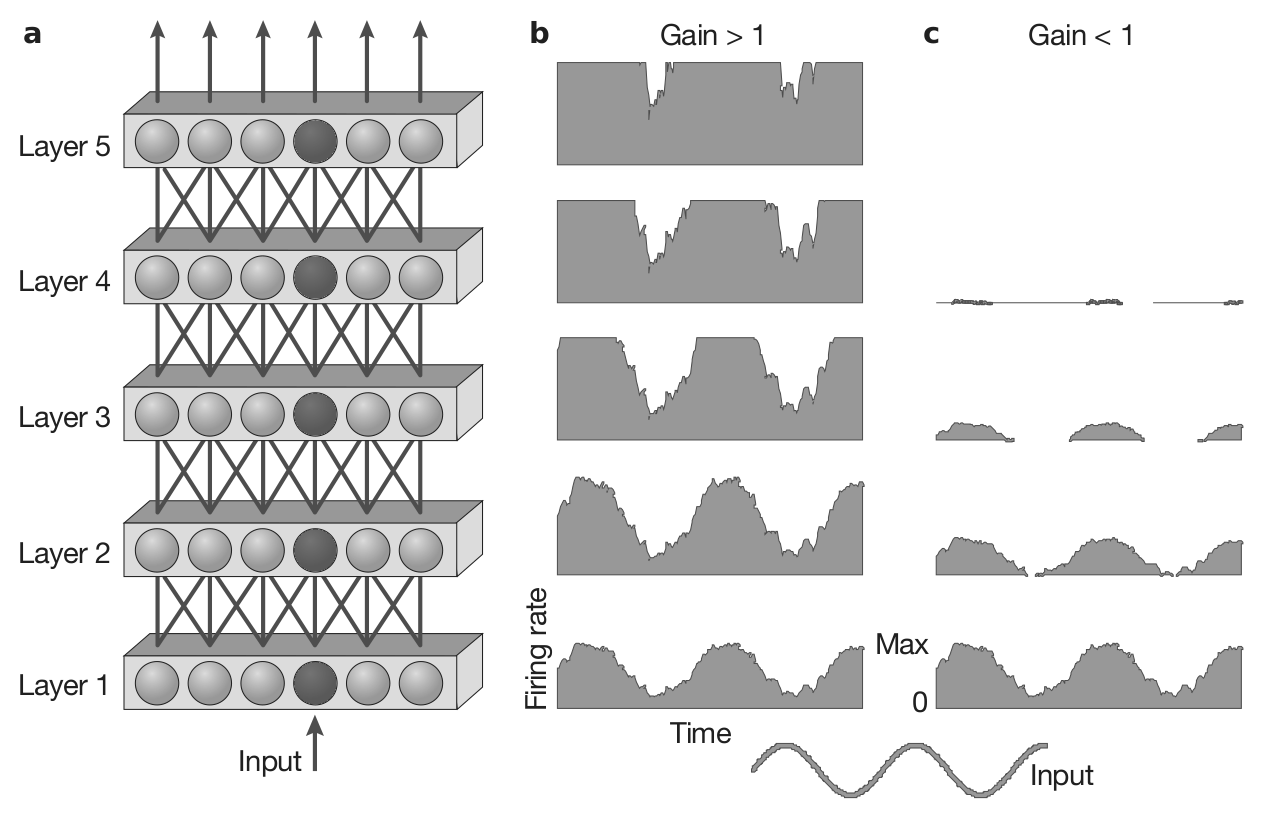
\includegraphics[width=0.6\textwidth]{neurons_plasticity/homeostatic-problem.png}
	\caption[Instability of networks]{Instability of networks for a simplified case \parencite[figure 1]{turrigiano2004homeostatic}. \textbf{a)} A small feed forward network with $5$ layers, the activity of the dark neuron is shown in b and c. \textbf{b)} If the gain is higher than $1$, the activity `explodes' and the sinusoidal input signal cannot be represented in the last layer. \textbf{c)} If the gain is lower than $1$, the signal `dies out' and is not able to reach the last layer.}
	\label{fig:homeo}
\end{figure}

\begin{itemize}
\item Type: Intrinsic (affecting the neuron) or synaptic (pre-synaptic and post-synaptic)
\item Spatial: More global (all synapses connected to a neuron) and more local or quasi-local (single synapse or small groups of synapses connected to a neuron)
\item Temporal: Fast (seconds to hours) and slow (hours to days)
\end{itemize}

\subsection{Synaptic normalization}
\label{sec:synaptic-scaling}

One important class of synaptic homeostatic plasticity is \emph{synaptic scaling}, where incoming synaptic connections to a neuron are normalized to a target weight. While adjusting the weights, their relative strengths are maintained. \textcite{turrigiano2008self} summarizes that neurons use calcium-dependent sensors to detect changes in their own firing rates. Depending on those changes the number of receptors at the synapses will be regulated. Note that the more local the mechanisms are and the fewer synapses are involved, the more the synaptic scaling mechanism will interact with \ac{ltd} and \ac{ltp} mechanisms, like \ac{stdp}.

While the normalizing process is highly complex in natural networks, in artificial systems it is relatively simple to perform. For example, in a simplified more global rule, every weight connected to a neuron $i$ is just normalized with all incoming weights from neurons $j$, using

\begin{equation}
\label{eq:sn}
w_{ij}(t) \leftarrow \frac{w_{ij}(t)}{\sum_{j=1}^N w_{ij}(t)},
\end{equation}

\nomenclature{$w_{ij}$}{Weight between neuron $i$ and neuron $j$}

where $w_{ij}(t)$ is the weight between neuron $i$ and $j$ at time $t$. Due to the mathematical process of normalization, it is also called \emph{synaptic normalization}.

\subsection{Intrinsic plasticity}
\label{sec:ip}

\ACFI{ip} is a process, which is local and intrinsic, since it only affects the conduction inside of a single neuron. In \acs{ip} no synapse and therefore, when modeling artificial networks, no weight is affected. There are several different types of \acl{ip} and many of them are not fully understood \parencite{cudmore2008intrinsic}. In principal, the neuron regulates biophysical properties of ion channels in the membrane. \textcite{awatramani2005modulation} showed that a small depolarization of about $10\,ms$ (resulting in a potential between $-60\,mV$ and $-65\,mV$), induced by a change of the extracellular concentration of calcium ions, enhances the probability of transmitter release up to $2$-fold.

\begin{wrapfigure}{R}{0.45\textwidth}
	\centering
	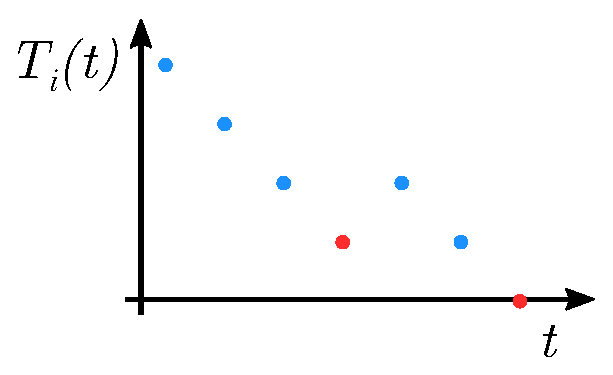
\includegraphics[width=0.45\textwidth]{neurons_plasticity/ip}
    \caption[Intrinsic plasticity and spontaneous activity]{Simple implementation of intrinsic plasticity. If the neuron is not spiking (blue dot), the threshold is decreased in the next step of time. If the neuron is spiking (red dot), the threshold is increased in the next step of time. If the threshold moves below zero, the neuron fires spontaneously.}
    \vspace{10pt}
    \label{fig:intrinsic-plasticity}
\end{wrapfigure}

A simple implementation in artificial neural networks affects the threshold for conducting the action potential inside of the neuron. If the neuron was active, the threshold will increase for the next step. If the neuron was not active, the threshold will decrease, to make the neuron more sensible. Note that if the threshold of a neuron becomes negative, the neuron fires spontaneously. The effect is shown in figure \ref{fig:intrinsic-plasticity}. The rule can be formalized with

\begin{equation}
\label{eq:ip}
T_i(t+1) = T_i(t) + \eta_\IP \left( x_i(t) - H_\IP \right),
\end{equation}

\nomenclature{$\eta_\IP$}{Learning rate for intrinsic plasticity}
\nomenclature{$T_i(t)$}{Threshold of neuron $i$ at time $t$}

where $\eta_\IP$ is the learning rate and $x_i(t) \in \{0,1\}$ the activity of neuron $i$ at time $t$. $H_\IP$ is the \emph{target rate}. All neurons will in average be active with a rate of $H_\IP$. The choice of $H_\IP$ is not trivial, since not all choices of the target rate will necessarily lead to a network with good performance \parencite{lazar2009sorn}.
